
\documentclass[a4paper,10pt]{article}
\usepackage[utf8x]{inputenc}
\usepackage[ngerman]{babel}
\usepackage[T1]{fontenc}      % T1-encoded fonts: auch Wörter mit Umlauten trennen
\usepackage{graphicx} 

%opening

\title{Schnittstellen- und Systementwurf}
\author{Rainer Hihn 19859\\Kathrin Holzmann 20228\\Florian Rosenkranz 19895}
\date{5.4.2011}
\begin{document}

\maketitle
\newpage
%\begin{abstract}

%\end{abstract}

\section{Inhalt}

\tableofcontents

\newpage

\section{Datenrahmen}

\begin{verbatim}
0             7              15              23
+-+-+-+-+-+-+-+-+-+-+-+-+-+-+-+-+-+-+-+-+-+-+-+
| Type        |  Length                       |
+-+-+-+-+-+-+-+-+-+-+-+-+-+-+-+-+-+-+-+-+-+-+-+
\end{verbatim}

\begin{tabbing}
 \hspace{2 cm}\=\kill
Type:\>uint8\_t, gibt die Art der Nachricht an\\
Length:\>uint16\_t, Länge der nachfolgenden Zusatzdaten in Bytes
\end{tabbing}

\subsection{Übersicht über die Nachrichtentypen}

\begin{verbatim}
 +------+------------------+----------------------------------------+---------+
| Type | Name             | Beschreibung                           | Richtg. |
+------+------------------+----------------------------------------+---------+
|    1 | LoginRequest     | Anmeldung des Clients am Server        | C ==> S |
+------+------------------+----------------------------------------+---------+
|    2 | LoginResponseOK  | Anmeldung am Server erfolgreich        | C <== S |
+------+------------------+----------------------------------------+---------+
|    3 | PlayerList       | Liste der Spielteilnehmer              | C <== S |
+------+------------------+----------------------------------------+---------+
|    4 | CatalogRequest   | Anforderung der Liste der Fragakata-   | C ==> S |
|      |                  | loge durch den Client                  |         |
+------+------------------+----------------------------------------+---------+
|    5 | CatalogResponse  | Name eines Fragekatalogs (mehrere      | C <== S |
|      |                  | Nachrichten dieses Typs ergeben die    |         |
|      |                  | vollständige Liste)                    |         |
+------+------------------+----------------------------------------+---------+
|    6 | CatalogChange    | Spielleiter hat Katalogauswahl ge-     | C <=> S |
|      |                  | ändert                                 |         |
+------+------------------+----------------------------------------+---------+
|    7 | StartGame        | Spielleiter möchte Spiel starten       | C <=> S |
+------+------------------+----------------------------------------+---------+
|    8 | QuestionRequest  | Anforderung einer Quizfrage durch      | C ==> S |
|      |                  | einen Client                           |         |
+------+------------------+----------------------------------------+---------+
|    9 | Question         | Transport einer Quiz-Frage zum Client  | C <== S |
+------+------------------+----------------------------------------+---------+
|   10 | QuestionAnswered | Quiz-Frage wurde beantwortet           | C ==> S |
+------+------------------+----------------------------------------+---------+
|   11 | QuestionResult   | Auswertung einer Antwort auf eine      | C <== S |
|      |                  | Quiz-Frage                             |         |
+------+------------------+----------------------------------------+---------+
|   12 | GameOver         | Alle Clients sind fertig, Mitteilung   | C <== S |
|      |                  | über Endplatzierung                    |         |
+------+------------------+----------------------------------------+---------+
|  255 | ErrorWarning     | Fehlermeldung an den Client            | C <== S |
+------+------------------+----------------------------------------+---------+
\end{verbatim}
Tabelle der Datenrahmentypen und deren Inhalt

\newpage

\section{Server}

\subsection{Login-Thread}

\subsubsection{Beschreibung}

Dieser Thread wird beim Starten des Servers geforked, das heißt automatisch mit gestartet. 
Sobald eine Anmeldung am Server erfolgreich ist, werden die nötigen Informationen an die Clientliste übertragen. 
Hierbei wird auch ein separater Client-Thread pro Client gestartet, dieser wartet nun auf Befehle.

\subsubsection{Datenrahmen}

LoginResponseOK

\begin{verbatim}
 0             7              15              23              31
+-+-+-+-+-+-+-+-+-+-+-+-+-+-+-+-+-+-+-+-+-+-+-+-+-+-+-+-+-+-+-+
| Type        | Length                        | Client-ID     |
+-+-+-+-+-+-+-+-+-+-+-+-+-+-+-+-+-+-+-+-+-+-+-+-+-+-+-+-+-+-+-+
\end{verbatim}

\begin{tabbing}
 \hspace{2 cm}\=\kill
Type:\>2\\
Length:\>1\\
Client-ID:\>uint8\_t, ID des Clients (0 := Spielleiter)
\end{tabbing}

$~~$ \\PlayerList\\ \\
Die folgende Nachricht wird aus Platzgründen verkürzt dargestellt. Das
Players-Feld ist immer 37*Spieleranzahl Bytes groß.

\begin{verbatim}
0             7              15              23              31
+-+-+-+-+-+-+-+-+-+-+-+-+-+-+-+-+-+-+-+-+-+-+-+-+-+-+-+-+-+-+-+
| Type        | Length                        | Players ..... =
+-+-+-+-+-+-+-+-+-+-+-+-+-+-+-+-+-+-+-+-+-+-+-+-+-+-+-+-+-+-+-+
= ........................................................... |
+-+-+-+-+-+-+-+-+-+-+-+-+-+-+-+-+-+-+-+-+-+-+-+-+-+-+-+-+-+-+-+
\end{verbatim}

\begin{tabbing}
 \hspace{2 cm}\=\kill
Type:\>3\\
Length:\>37*Spieleranzahl (maximal 6*37 = 222)\\ 
Players:\>Liste aller derzeit angemeldeten Benutzer
\end{tabbing}

\newpage

$~~$\\ErrorWarning

\begin{verbatim}
 0             7              15              23              31
+-+-+-+-+-+-+-+-+-+-+-+-+-+-+-+-+-+-+-+-+-+-+-+-+-+-+-+-+-+-+-+
| Type        | Length                        | Subtype       |
+-+-+-+-+-+-+-+-+-+-+-+-+-+-+-+-+-+-+-+-+-+-+-+-+-+-+-+-+-+-+-+
| [Message] ................................................. |
+-+-+-+-+-+-+-+-+-+-+-+-+-+-+-+-+-+-+-+-+-+-+-+-+-+-+-+-+-+-+-+
\end{verbatim}

\begin{tabbing}
 \hspace*{2 cm}\=\\=\kill
Type:\>255\\
Length:\>1 + Länge(Message)\\
Subtype:\>uint8\_t\\
\>0 -> fataler Fehler\\
\>1 -> Warnung\\
Message:\>Beschreibung des Fehlers im Textformat (UTF-8), nicht nullterminiert
\end{tabbing}

\subsubsection{Ablaufdiagramm}

\begin{center}
 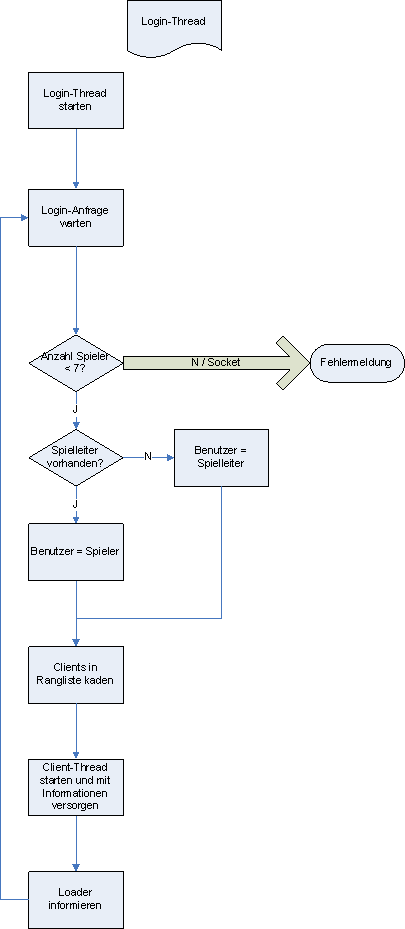
\includegraphics[scale=0.5]{../YDKR/doku/Abgabe3/Login-Thread.png}
 % login-thread.png: 405x990 pixel, 72dpi, 14.29x34.92 cm, bb=0 0 405 990
\end{center}

Ablaufdiagramm Login-Thread

\subsection{PlayerList}

\subsubsection{Beschreibung}

Speicherung und Verwaltung wichtiger Informationen, die für die Clientkommunikation nötig sind. Während der Spielphase muss der Server diese Liste absteigend nach
den Punkteständen der Spieler sortieren.

\subsubsection{Aufbau}

\begin{tabbing}
\hspace{2 cm}\=\kill
32 Bytes\>Spielername X (UTF-8, nullterminiert)\\
4 Bytes\>Punktestand Spieler X, vorzeichenlos\\
1 Byte\>ID Spieler X\\
\>…
\end{tabbing}


\subsection{Client-Thread}

\subsubsection{Beschreibung}

Der Client-Thread ist die wichtigste Schnittstelle zum Client. Für Jeden der angemeldeten Clients gibt es einen Client-Thread. 
Die Identifizierung wird über die ClientID zugewiesen


\subsubsection{Datenrahmen}

CatalogResponse

\begin{verbatim}
 0             7              15              23              31
+-+-+-+-+-+-+-+-+-+-+-+-+-+-+-+-+-+-+-+-+-+-+-+-+-+-+-+-+-+-+-+
| Type        | Length                        | [Filename] .. |
+-+-+-+-+-+-+-+-+-+-+-+-+-+-+-+-+-+-+-+-+-+-+-+-+-+-+-+-+-+-+-+
\end{verbatim}

\begin{tabbing}
\hspace{2 cm}\=\kill
Type:\>5\\
Length:\>Länge des Dateinamens, oder 0 für Endemarkierung\\
Filename:\>Dateiname eines Fragekataloges (UTF-8, nicht nullterminiert), oder leer für Endemarkierung
\end{tabbing}

$~~$\\StartGame
\begin{verbatim}
 0             7              15              23              31
+-+-+-+-+-+-+-+-+-+-+-+-+-+-+-+-+-+-+-+-+-+-+-+-+-+-+-+-+-+-+-+
| Type        | Length                        | [Filename] .. |
+-+-+-+-+-+-+-+-+-+-+-+-+-+-+-+-+-+-+-+-+-+-+-+-+-+-+-+-+-+-+-+
\end{verbatim}

\begin{tabbing}
\hspace{2 cm}\=\kill
Type:\>7\\
Length:\>Länge des Dateinamens\\
Filename:\>Dateiname des zu spielenden Fragekataloges (UTF-8, nicht nullterminiert), \\
\>kann beim Versand Server ==> Client (nicht Client ==> Server!) auch leer gelassen werden
\end{tabbing}

$~~$\\Question\\\\
Die folgende Nachricht wird aus Platzgründen verkürzt dargestellt. Wenn
Fragedaten versendet werden (also nicht die Nachricht verschickt wird, dass es
keine Fragen mehr gibt), dann ist das Data-Feld genau 770 Bytes groß.

\begin{verbatim}
 0             7              15              23              31
+-+-+-+-+-+-+-+-+-+-+-+-+-+-+-+-+-+-+-+-+-+-+-+-+-+-+-+-+-+-+-+
| Type        | Length                        | [Data] ...... =
+-+-+-+-+-+-+-+-+-+-+-+-+-+-+-+-+-+-+-+-+-+-+-+-+-+-+-+-+-+-+-+
= ............................................................|
+-+-+-+-+-+-+-+-+-+-+-+-+-+-+-+-+-+-+-+-+-+-+-+-+-+-+-+-+-+-+-+
\end{verbatim}

\begin{tabbing}
\hspace{2 cm}\=\kill
Type:\>9\\
Length:\>770 oder 0 (falls keine Fragen mehr)\\
Data:\>Eine Struktur, die wie unten angegeben aufgebaut ist, oder leer (falls keine Fragen mehr)
\end{tabbing}

\begin{tabbing}
\hspace{2 cm}\=\kill
Aufbau des Data-Felds:\\
256 Bytes\>Text der Fragestellung (UTF-8, nullterminiert)\\
128 Bytes\>Antworttext 1 (UTF-8, nullterminiert)\\
128 Bytes\>Antworttext 2 (UTF-8, nullterminiert)\\
128 Bytes\>Antworttext 3 (UTF-8, nullterminiert)\\
128 Bytes\>Antworttext 4 (UTF-8, nullterminiert)\\
\ \  \ 2 Bytes\>Zeitbegrenzung in Sekunden, vorzeichenlos, in Network Byte Order
\end{tabbing}


$~~$\\QuestionResult

\begin{verbatim}
 0             7              15              23              31
+-+-+-+-+-+-+-+-+-+-+-+-+-+-+-+-+-+-+-+-+-+-+-+-+-+-+-+-+-+-+-+
| Type        | Length                        | Selection     |
+-+-+-+-+-+-+-+-+-+-+-+-+-+-+-+-+-+-+-+-+-+-+-+-+-+-+-+-+-+-+-+
| Correct     |
+-+-+-+-+-+-+-+
\end{verbatim}

\begin{tabbing}
\hspace{2 cm}\=\kill
Type:\>11\\
Length:\>2\\
Selection:\>uint8\_t, Index der zuvor vom Benutzer gewählten Antwort\\
\>(0 <= Selection <= 3), oder 255 falls Zeit für Frage abgelaufen
\end{tabbing}

$~~$\\GameOver

\begin{verbatim}
 0             7              15              23              31
+-+-+-+-+-+-+-+-+-+-+-+-+-+-+-+-+-+-+-+-+-+-+-+-+-+-+-+-+-+-+-+
| Type        | Length                        | Rank          |
+-+-+-+-+-+-+-+-+-+-+-+-+-+-+-+-+-+-+-+-+-+-+-+-+-+-+-+-+-+-+-+
\end{verbatim}

\begin{tabbing}
\hspace{2 cm}\=\kill
Type:\>12\\
Length:\>1\\
Selection:\>uint8\_t, Endposition des Benutzers in der Rangliste (1 <= Rank <= 6)\\
\end{tabbing}

\subsubsection{Ablaufdiagramm}
\begin{center}
 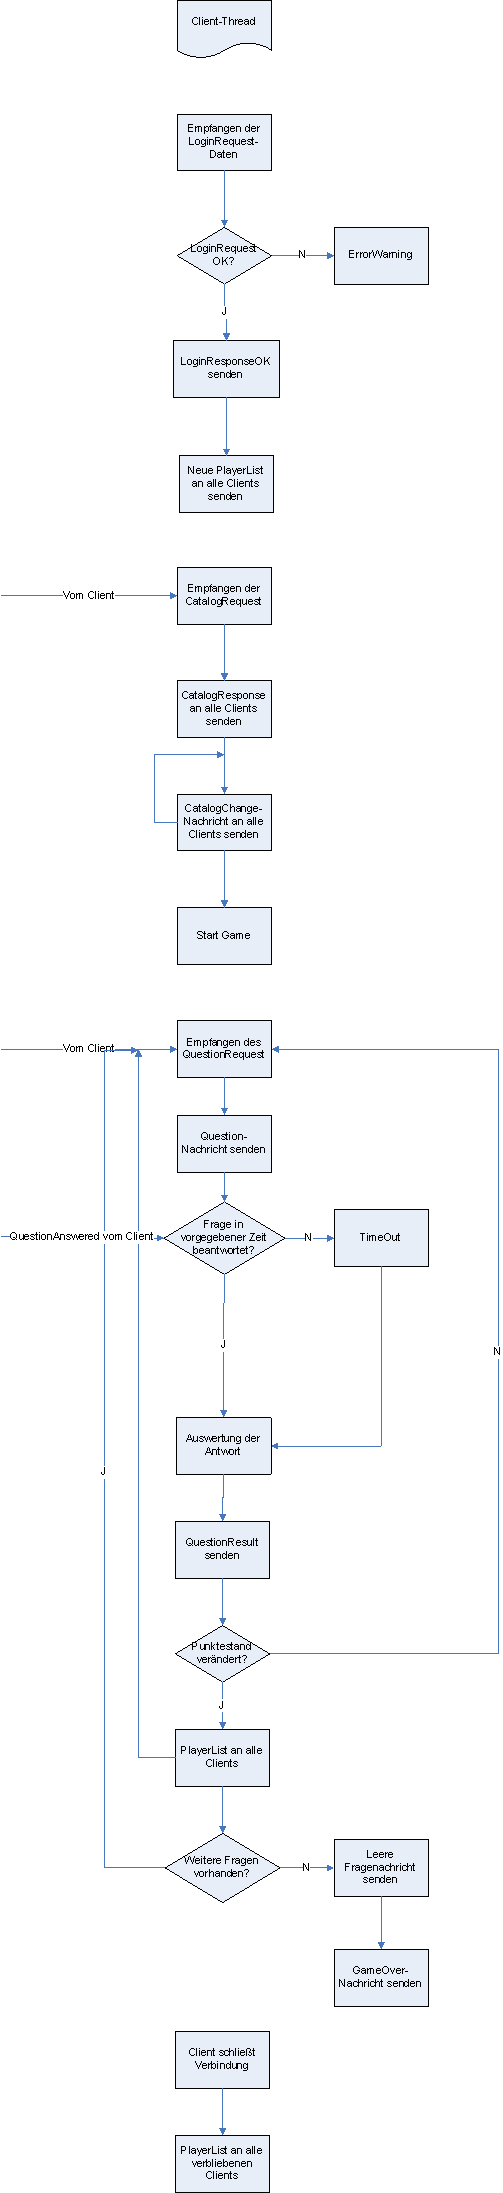
\includegraphics[scale=0.25]{../YDKR/doku/Abgabe3/Client-Thread.png}
 % login-thread.png: 405x990 pixel, 72dpi, 14.29x34.92 cm, bb=0 0 405 990
\end{center}
Ablaufdiagramm Client-Thread

\subsection{Loader}

Erhält durch den Client-Thread Loader-Kommandos und führt eine Aktion mit anschließender Antwort aus.

\begin{center}
\begin{tabular}{|l|l|}\hline
\textbf{Kommando} & \textbf{Bedeutung}\\\hline
LOAD & Fragenkatalog in den Shared Memory Laden\\\hline
BROWSE & Liste aller Fragenkataloge auf der Standardausgabe ausgeben\\\hline
\end{tabular}
\end{center}

\begin{center}
\begin{tabular}{|l|l|}\hline
\textbf{Meldung} & \textbf{Bedeutung}\\\hline
LOADED, SIZE = n & Katalog mit n Fragen erfolgreich geladen\\\hline
ERROR: CANNOT OPEN FILE & Fragenkatalog konnte nicht geöffnet werden\\\hline
ERROR: CANNOT READ FILE & Fehler beim Lesen aus dem Fragenkatalog\\\hline
ERROR: INVALID CATALOG & Übergebene Datei ist kein gültiger Fragenkatalog\\\hline
ERROR: CANNOT USE SHARED MEMORY & Fehler bei der Verwendung des Shared Memory\\\hline
ERROR: OUT OF MEMORY & Zu wenig freier Hauptspeicher\\\hline
\end{tabular}
\end{center}

$~~$\\Übernommen aus “Systemprogrammierung unter Linux, Client- Server Projekt Multiplayer Quiz” Seite 8

\section{Client}

\subsection{Command-Thread}

\subsubsection{Beschreibung}

Besitzt die eigentliche Verbindung zum Client-Thread des Servers. Somit besteht eine eindeutige Socketverbindung zwischen Client und Server. 
Der Command-Thread sendet die eigentlichen Befehle aus Server- oder Client-Thread an den Server. 

\subsubsection{Datenrahmen}

LoginRequest

\begin{verbatim}
 0             7              15              23              31
+-+-+-+-+-+-+-+-+-+-+-+-+-+-+-+-+-+-+-+-+-+-+-+-+-+-+-+-+-+-+-+
| Type        | Length                        | Name ........ |
+-+-+-+-+-+-+-+-+-+-+-+-+-+-+-+-+-+-+-+-+-+-+-+-+-+-+-+-+-+-+-+
\end{verbatim}

\begin{tabbing}
\hspace{2 cm}\=\kill
Type:\>1\\
Length:\>Länge des Namens (Length <= 31)\\
Name:\>Login-Name, UTF-8, nicht nullterminiert, maximal 31 Bytes\\
\end{tabbing}

$~~$\\CatalogRequest

\begin{verbatim}
0             7              15              23
+-+-+-+-+-+-+-+-+-+-+-+-+-+-+-+-+-+-+-+-+-+-+-+
| Type        | Length                        |
+-+-+-+-+-+-+-+-+-+-+-+-+-+-+-+-+-+-+-+-+-+-+-+
\end{verbatim}

\begin{tabbing}
\hspace{2 cm}\=\kill
Type:\>4\\
Length:\>0\\
\end{tabbing}

$~~$\\CatalogChange

\begin{verbatim}
0             7              15              23              31
+-+-+-+-+-+-+-+-+-+-+-+-+-+-+-+-+-+-+-+-+-+-+-+-+-+-+-+-+-+-+-+
| Type        | Length                        | Filename .... |
+-+-+-+-+-+-+-+-+-+-+-+-+-+-+-+-+-+-+-+-+-+-+-+-+-+-+-+-+-+-+-+
\end{verbatim}

\begin{tabbing}
\hspace{2 cm}\=\kill
Type:\>6\\
Length:\>Länge des Dateinamens\\
Filename:\>Dateiname des gewählten Fragekataloges (UTF-8, nicht nullterminiert)\\
\end{tabbing}


$~~$\\StartGame

\begin{verbatim}
0             7              15              23              31
+-+-+-+-+-+-+-+-+-+-+-+-+-+-+-+-+-+-+-+-+-+-+-+-+-+-+-+-+-+-+-+
| Type        | Length                        | [Filename] .. |
+-+-+-+-+-+-+-+-+-+-+-+-+-+-+-+-+-+-+-+-+-+-+-+-+-+-+-+-+-+-+-+
\end{verbatim}

\begin{tabbing}
\hspace{2 cm}\=\kill
Type:\>7\\
Length:\>Länge des Dateinamens\\
Filename:\>Dateiname des zu spielenden Fragekataloges (UTF-8, nicht nullterminiert), \\
\>kann beim Versand Server ==> Client (nicht Client ==> Server!) \\
\>auch leer gelassen werden\\
\end{tabbing}

$~~$\\QuestionAnswered

\begin{verbatim}
0             7              15              23              31
+-+-+-+-+-+-+-+-+-+-+-+-+-+-+-+-+-+-+-+-+-+-+-+-+-+-+-+-+-+-+-+
| Type        | Length                        | Selection     |
+-+-+-+-+-+-+-+-+-+-+-+-+-+-+-+-+-+-+-+-+-+-+-+-+-+-+-+-+-+-+-+
\end{verbatim}

\begin{tabbing}
\hspace{2 cm}\=\kill
Type:\>10\\
Length:\>1\\
Selection:\>uint8\_t, Index der vom Benutzer gewählten Antwortmöglichkeit (0 <= Selection <= 3)\\
\end{tabbing}

\subsubsection{Ablaufdiagramm}

\begin{center}
 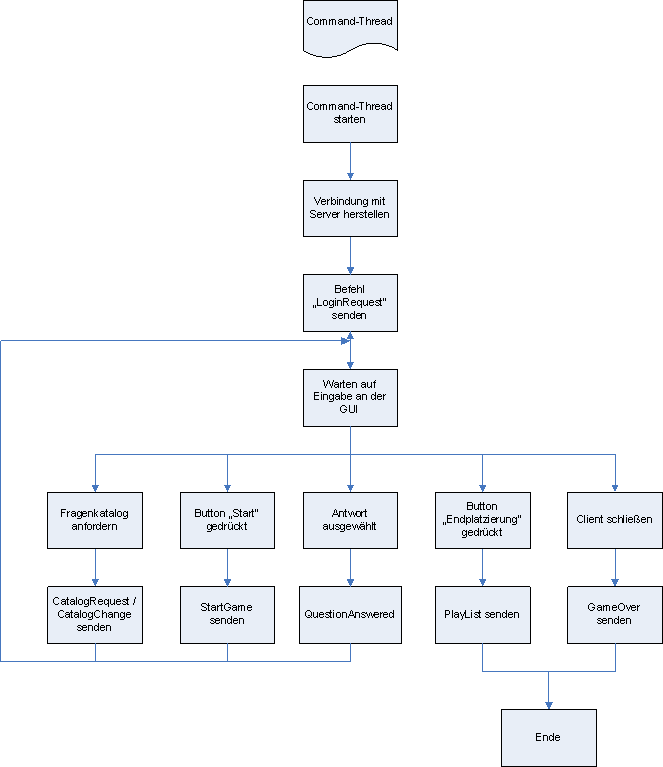
\includegraphics[scale=0.5]{../YDKR/doku/Abgabe3/Command-Thread.png}
 % login-thread.png: 405x990 pixel, 72dpi, 14.29x34.92 cm, bb=0 0 405 990
\end{center}

Ablaufdiagramm Command-Thread

\subsection{Fragewechsel-Thread}

\subsubsection{Beschreibung}

Verantwortlich für die Wartezeit zwischen den Fragen und das Anfordern neuer Fragen.

\subsubsection{Datenrahmen}

QuestionRequest

\begin{verbatim}
0             7              15              23
+-+-+-+-+-+-+-+-+-+-+-+-+-+-+-+-+-+-+-+-+-+-+-+
| Type        | Length                        |
+-+-+-+-+-+-+-+-+-+-+-+-+-+-+-+-+-+-+-+-+-+-+-+
\end{verbatim}

\begin{tabbing}
\hspace{2 cm}\=\kill
Type:\>8\\
Length:\>0\\
\end{tabbing}

\subsubsection{Ablaufdiagramm}

\begin{center}
 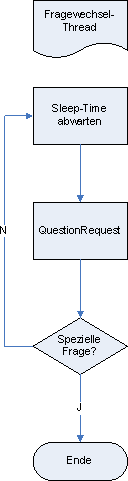
\includegraphics[scale=0.5]{../YDKR/doku/Abgabe3/Fragewechsel-Thread.png}
 % login-thread.png: 405x990 pixel, 72dpi, 14.29x34.92 cm, bb=0 0 405 990
\end{center}

Ablaufdiagramm Fragewechsel-Thread

\subsection{Listener-Thread}

\subsubsection{Beschreibung}

Dieser Thread achtet auf Broadcasts vom Server zur Aktualisierung des Punktestands. Außerdem achtet er auf die Eingaben der Benutzer.

\subsubsection{Ablaufdiagramm}

\begin{center}
 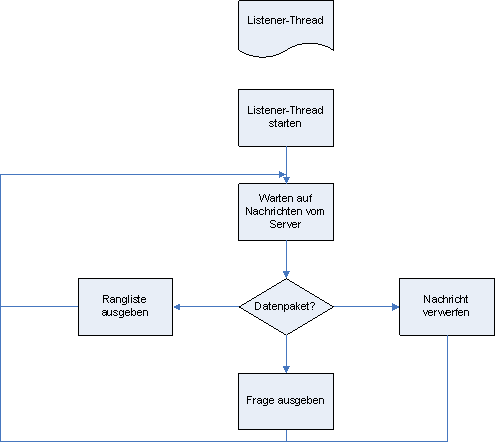
\includegraphics[scale=0.5]{../YDKR/doku/Abgabe3/Listener-Thread.png}
 % login-thread.png: 405x990 pixel, 72dpi, 14.29x34.92 cm, bb=0 0 405 990
\end{center}

Ablaufdiagramm Listener-Thread

\section{Projektteam}

\subsection{Zusammensetzung}

\begin{tabbing}
\hspace{3,5 cm}\=\kill
Teammitglieder:\>Rainer Hihn, Kathrin Holzmann, Florian Rosenkranz\\
Teamleiter:\>Kathrin Holzmann\\
\end{tabbing}


\subsection{Aufgabenverteilung}

\begin{tabbing}
\hspace{3,5 cm}\=\kill
Rainer Hihn:\>Login,Vorbereiteung, Doku\\
Kathrin Holzmann:\>Spiel, Spielende, Logout, Doku\\
Florian Rosenkranz:\>Spiel, Spielende, Logout, Doku\\
\end{tabbing}









\end{document}
